\section{Doppelbelichtung}
\subsection{Versuchsbeschreibung}

Bei der Doppelbelichtungstechnik wird ein Hologramm des zu untersuchenden Objekts aufgenommen. Dabei befindet sich dieses während einer Hälfte der Belichtungszeit im ersten Zustand und wird dann für den Rest der Zeit in den zweiten Zustand gebracht. Man sieht dann im fertigen Hologramm die Interferenz beider Zustände.

In unserem Fall soll das Biegeverhalten von Metallstäben untersucht werden. Diese werden dazu sowohl mit als auch ohne einem ziehenden Gewicht aufgenommen. Aus dem Interferenzmuster können dann die Weglängenunterschiede und somit die Biegung der Stäbe ermittlelt werden. 

\subsection{Durchführung und Auswertung}

%TODO: blabla bla blabla

\begin{figure}[ht]
 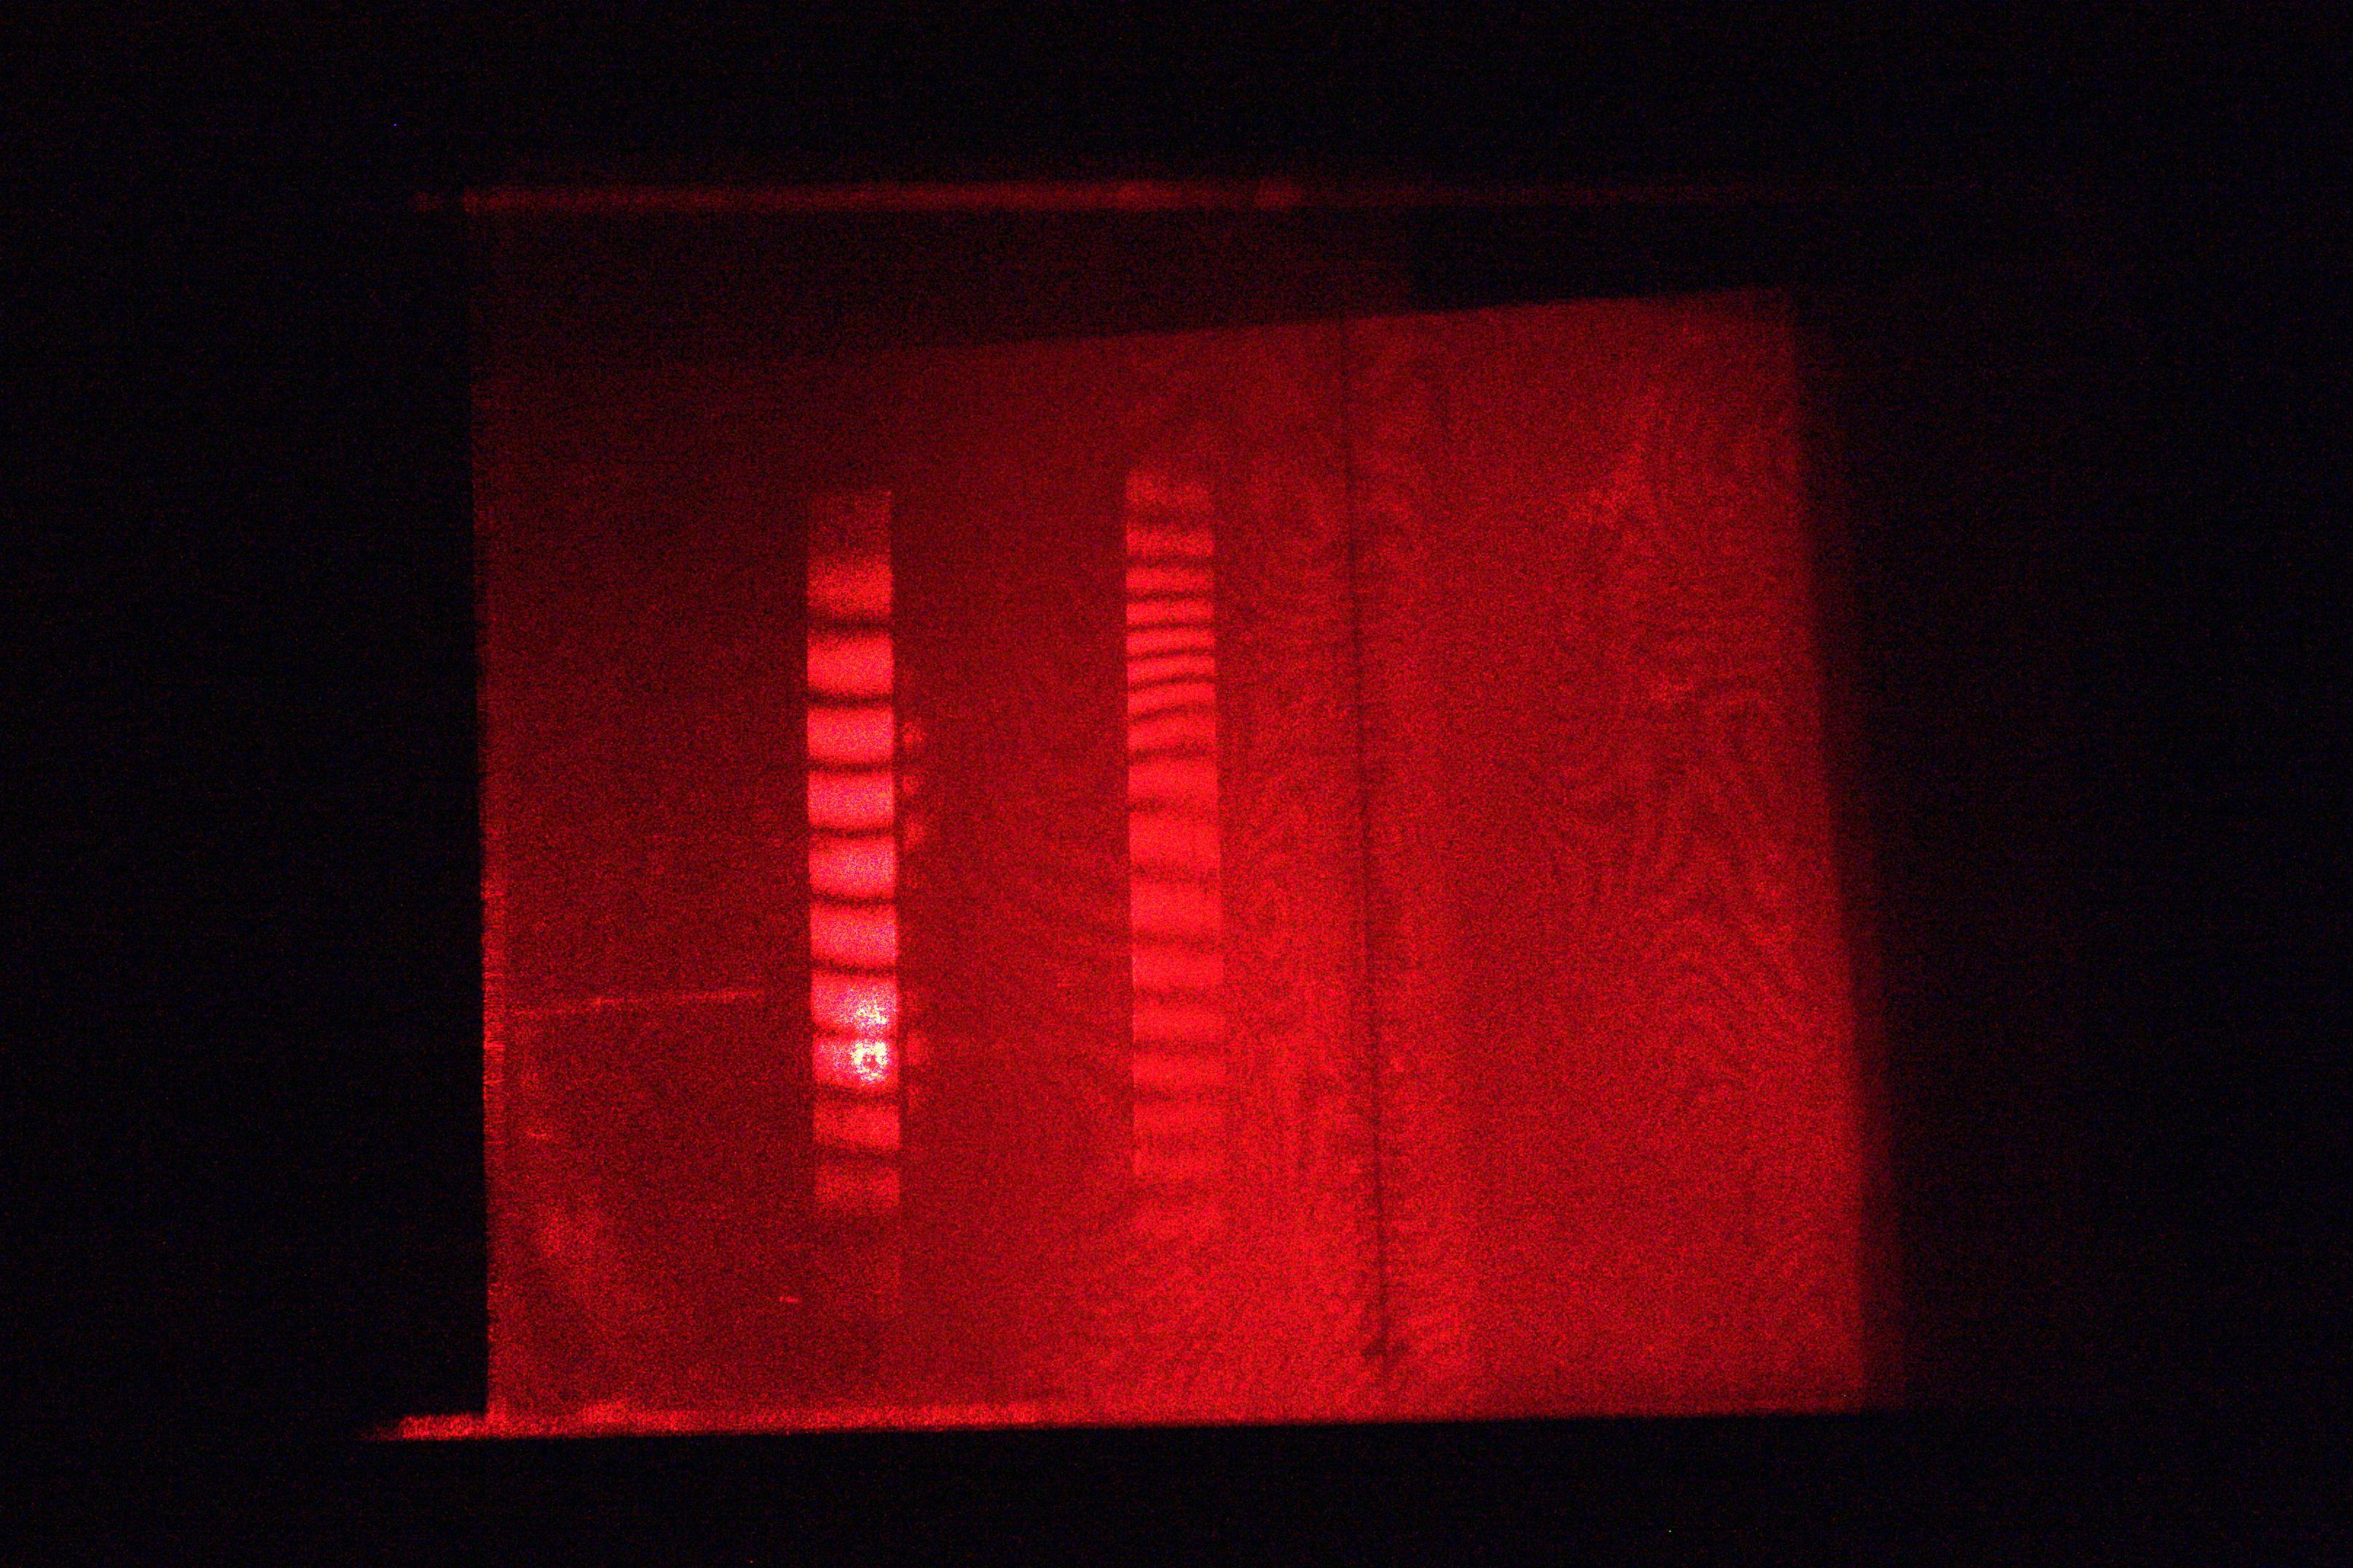
\includegraphics[width=\textwidth]{Photos/IMG_3909.jpg}
 \caption{Hologramm der linken beiden Stäbe}
\end{figure}


\begin{figure}[ht]
 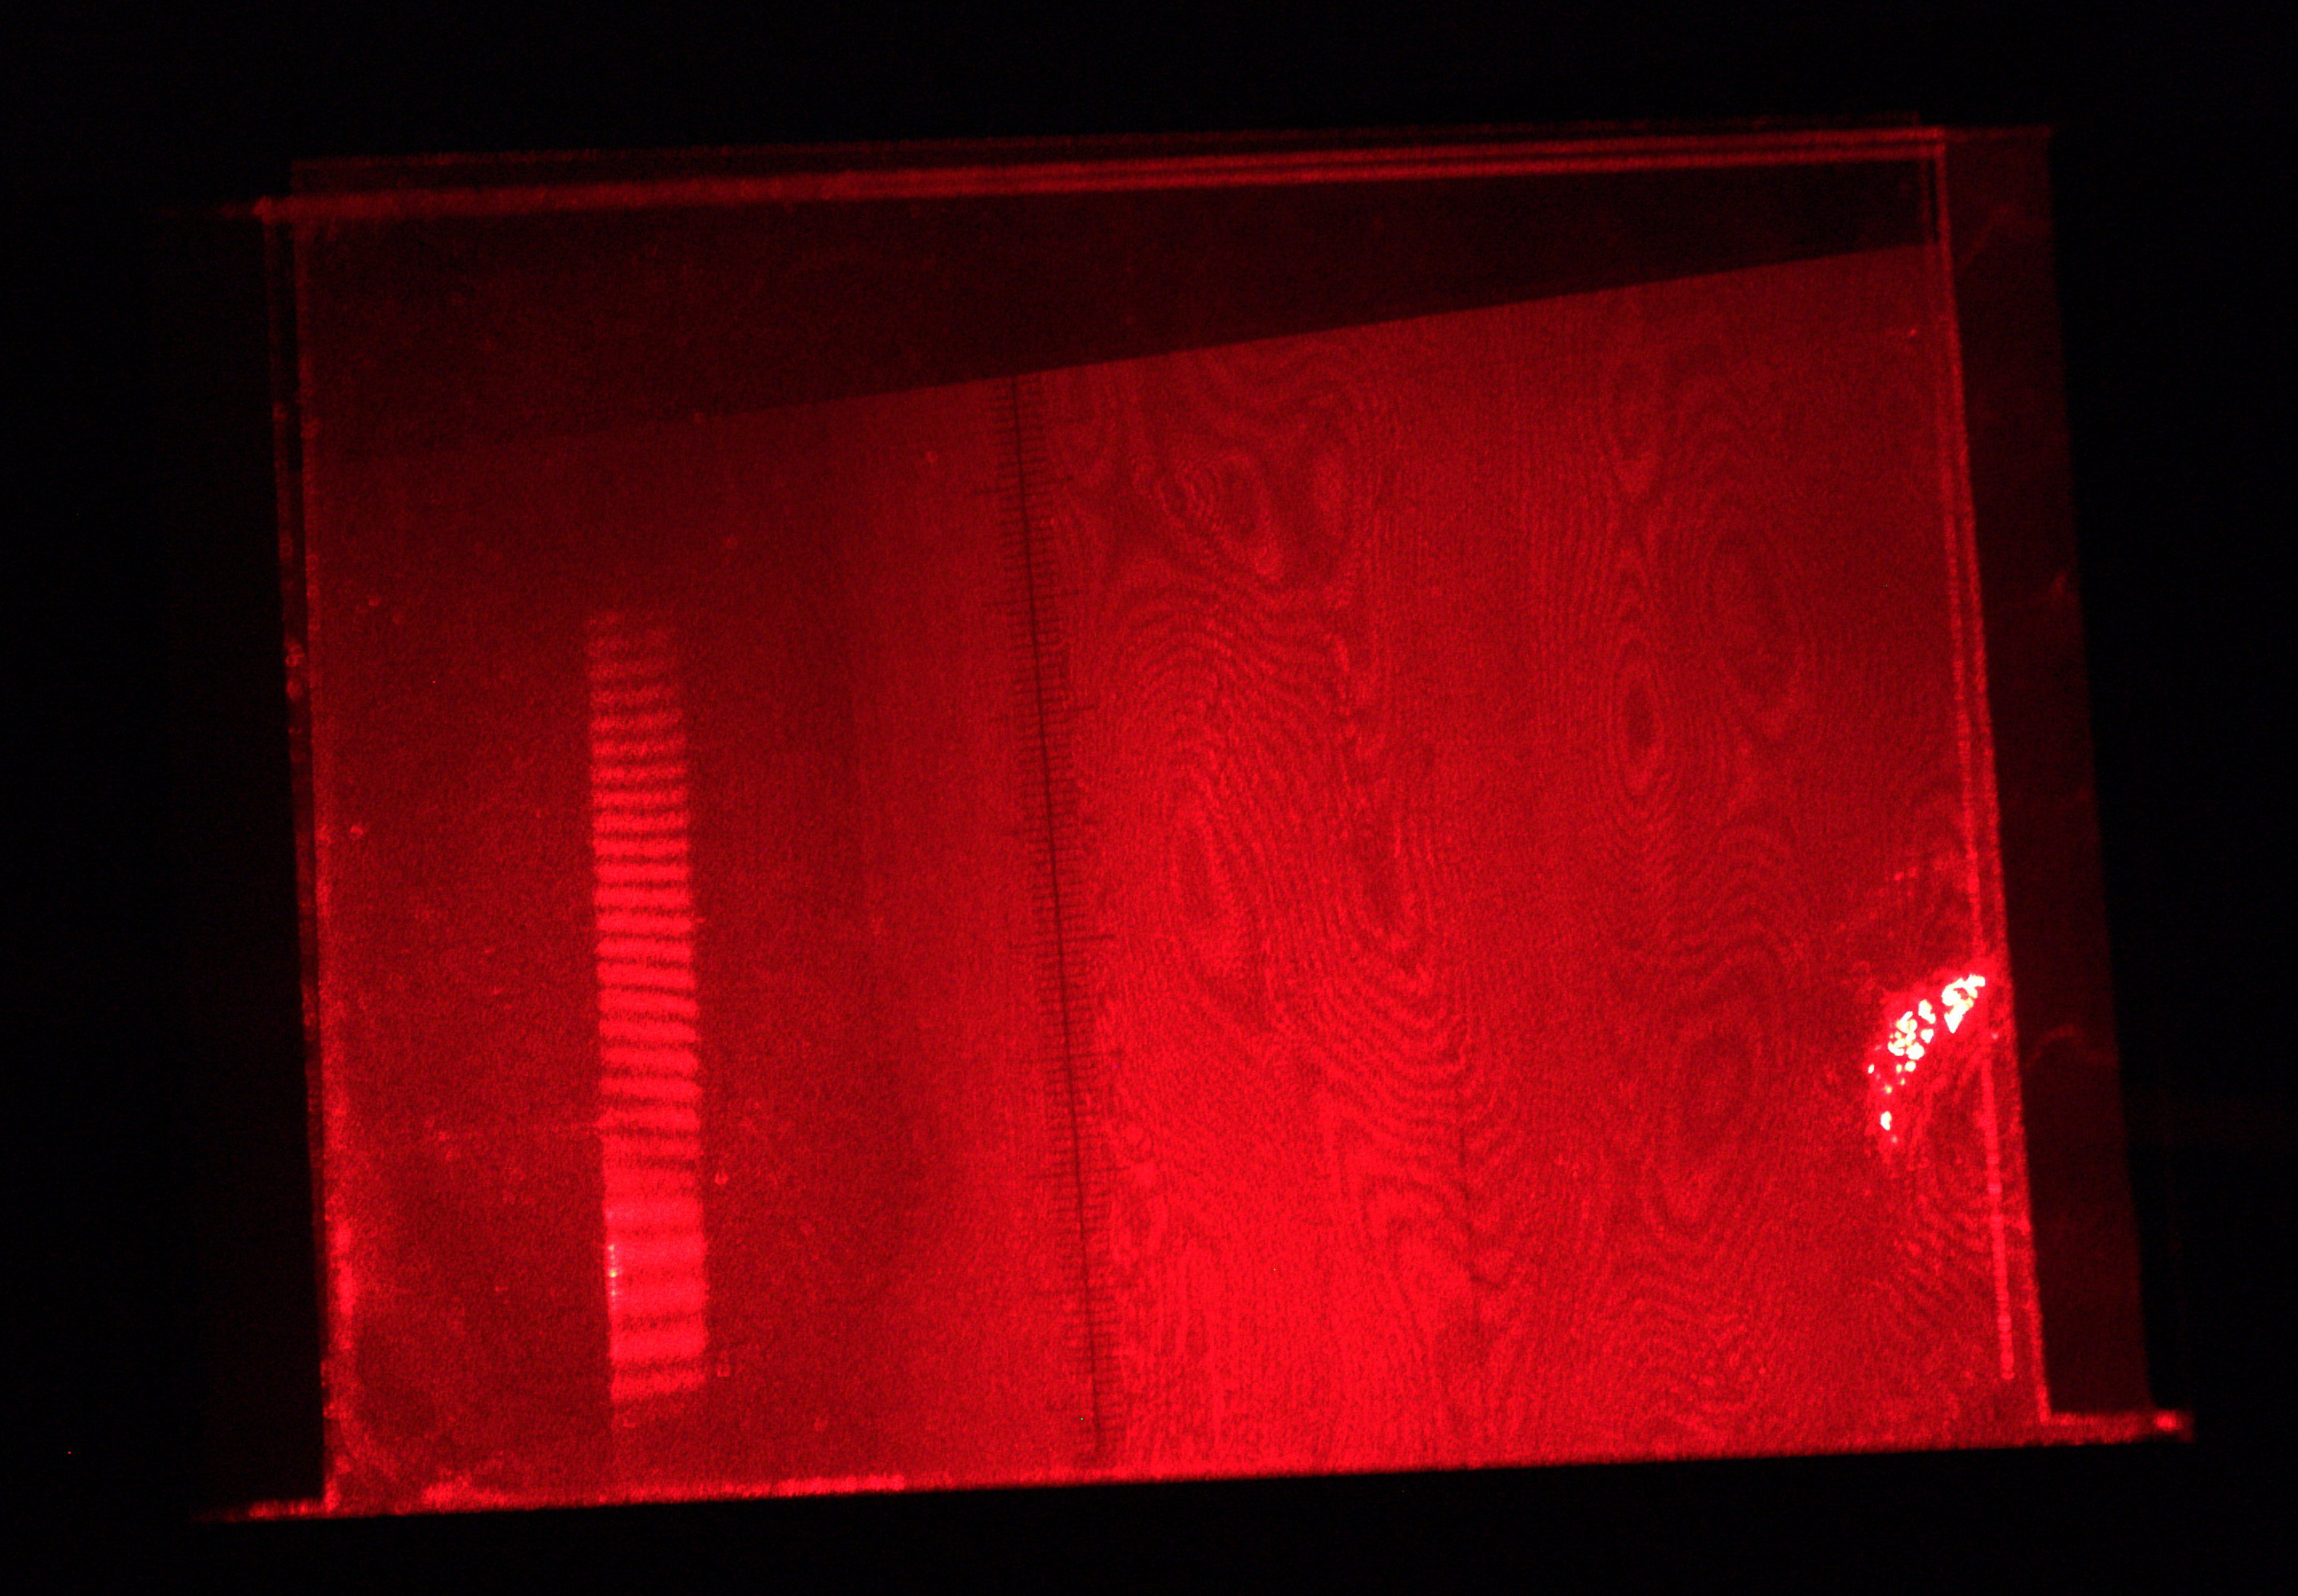
\includegraphics[width=\textwidth]{Photos/IMG_3919.jpg}
 \caption{Hologramm des rechten Stabes}
\end{figure}

\begin{figure}[ht]
 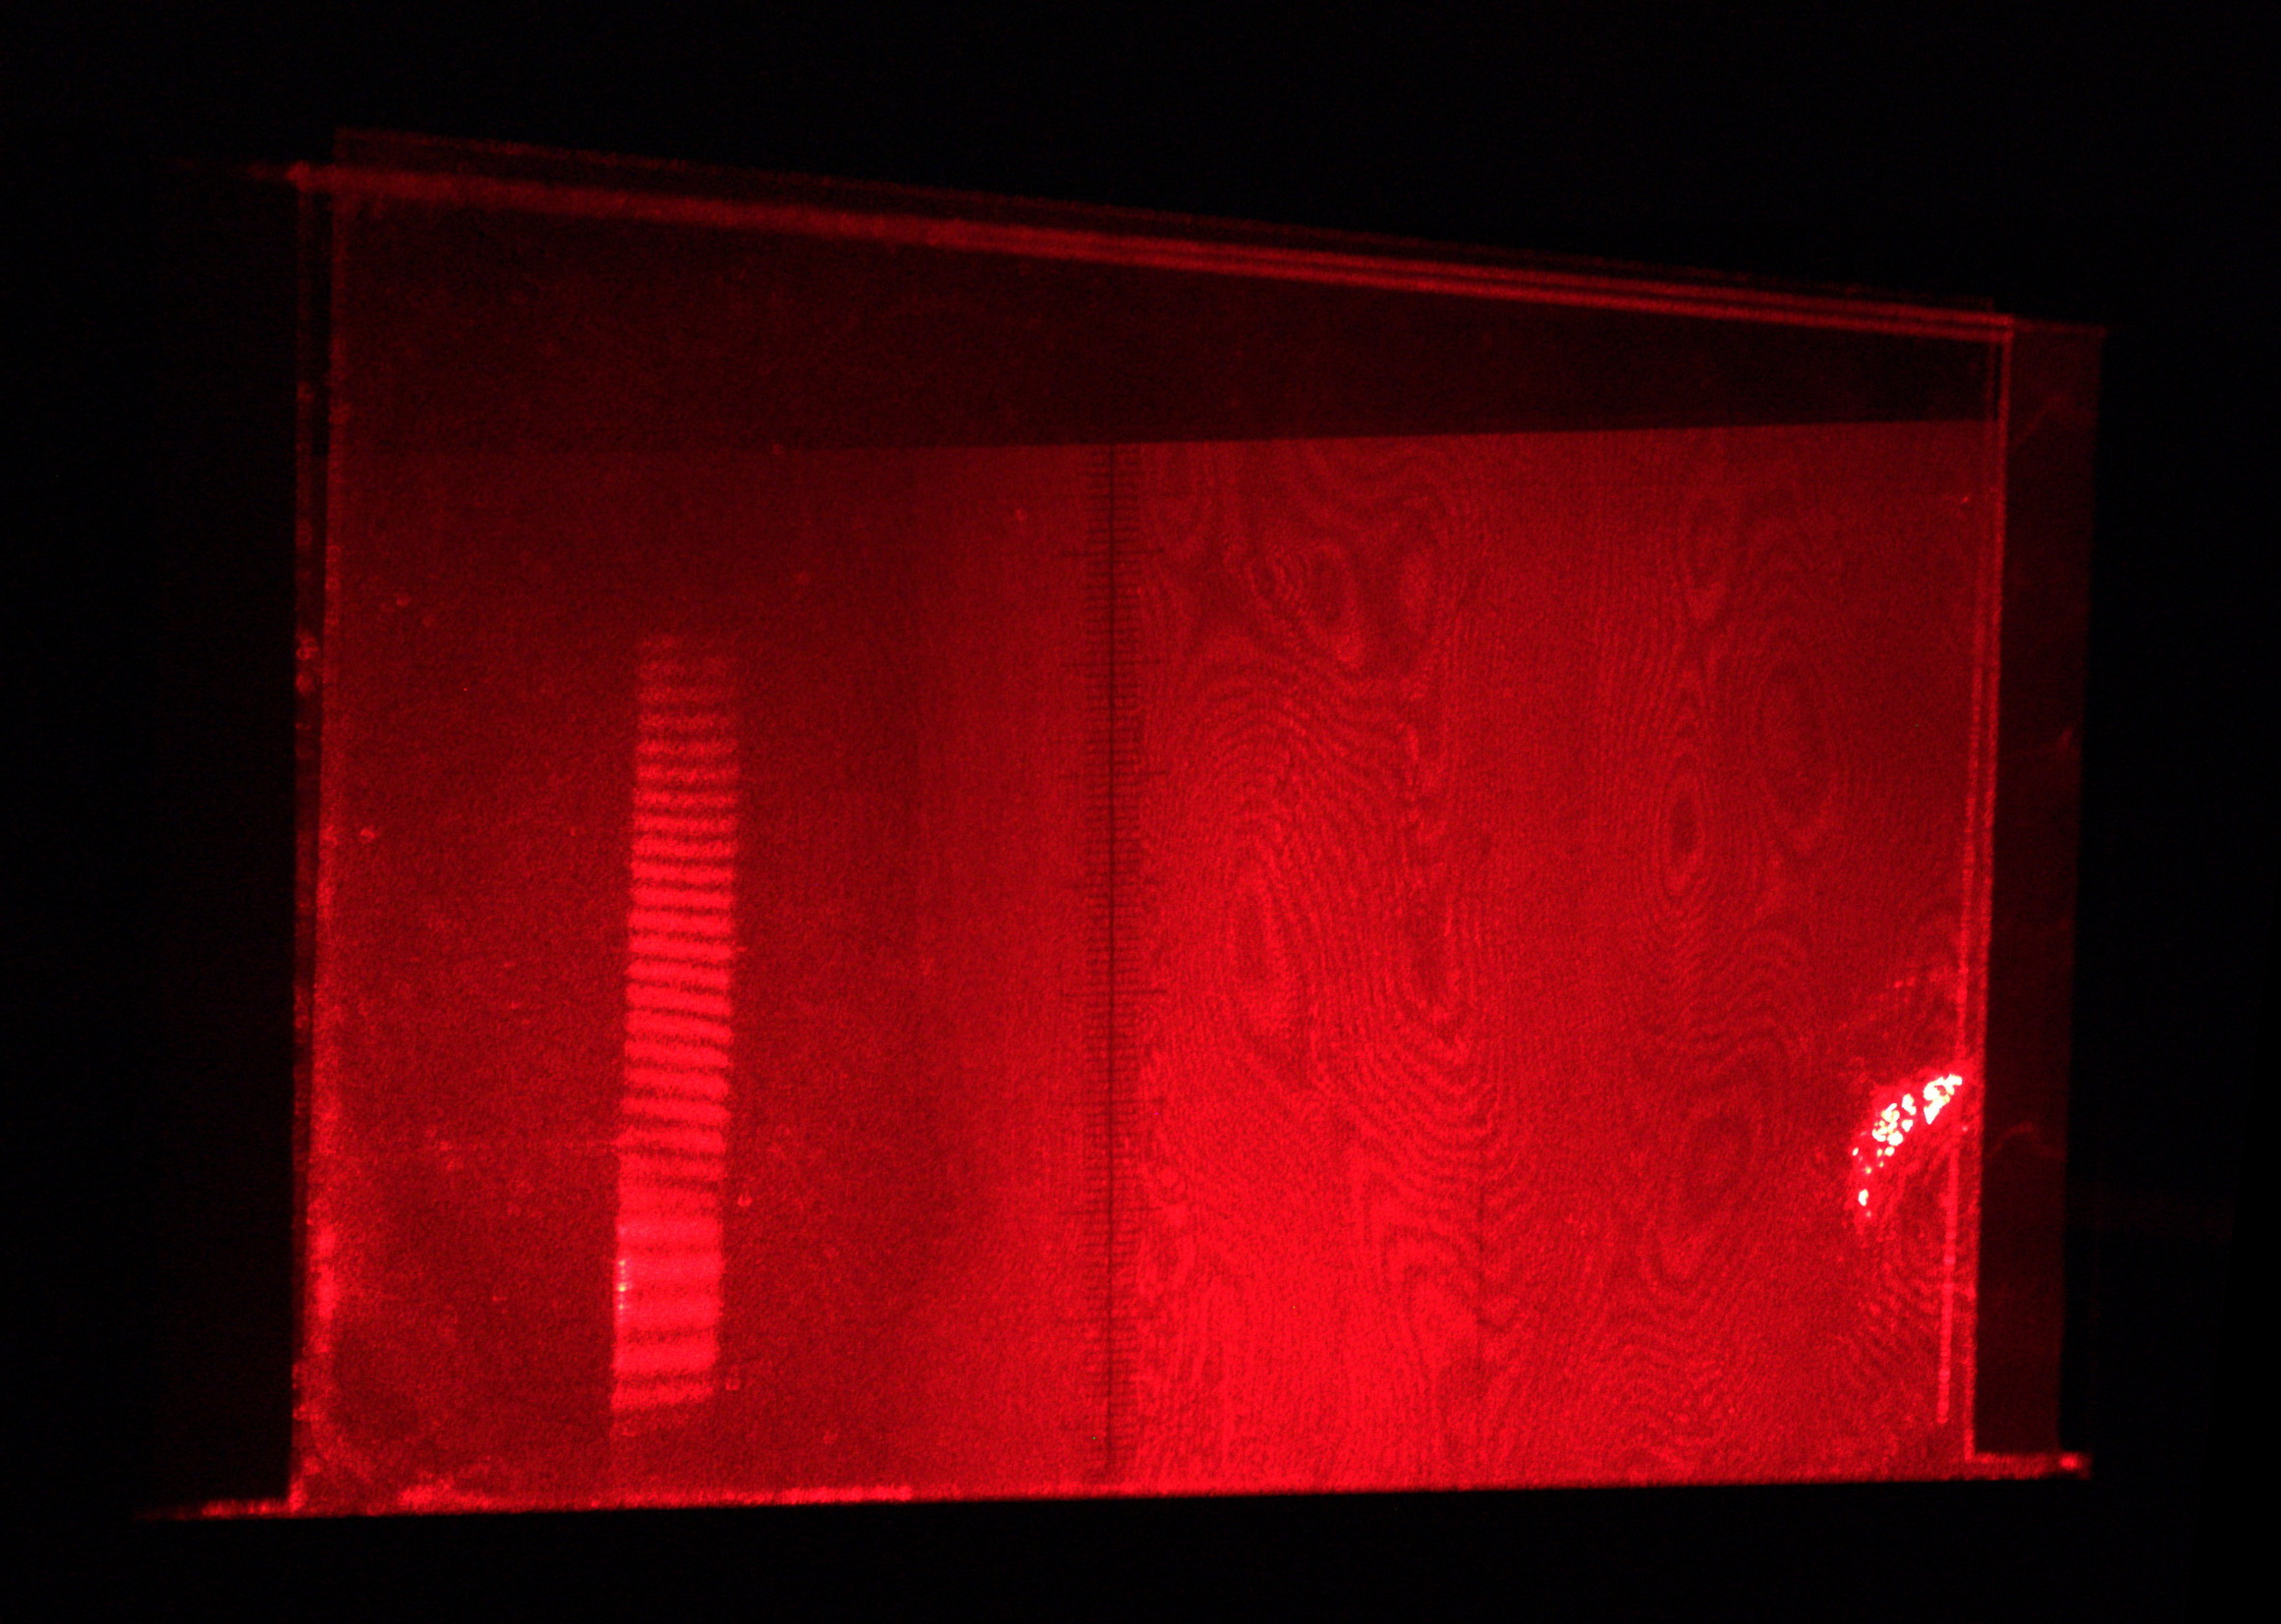
\includegraphics[width=\textwidth]{Photos/IMG_3919-korrigiert.jpg}
 \caption{Hologramm des rechten Stabes mit Perspektivenkorrektur}
\end{figure}

Das erste Minimum des Interferenzmusters ausgehend von der Befestigung entspricht einer Differenz von $\Delta x_1 = \nicefrac{\lambda}{2}$, die weiteren Minimas liegen dann bei $\Delta x_i = \Delta x_{i-1} + \lambda$. Wir haben also mit dem Programm {\verb Engauge Digitizer} über die Skala des Schirms die Position der Minima abgelesen und die Verbiegung berechnet. 

%TODO: Balken vermessen!

\begin{figure}[ht]
 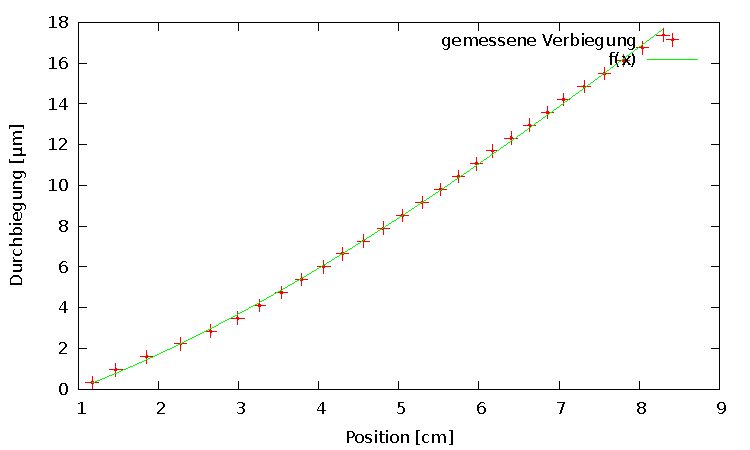
\includegraphics[width=\textwidth]{Graphen/biegung-balken3.pdf}
 \caption{Durchbiegung des Aluminium-Stabes}
\end{figure}
  